\documentclass{beamer}
\usepackage{animate}
\usepackage{multimedia}
\usepackage[english,russian]{babel}

\usepackage{pgfpages}
\setbeameroption{show notes on second screen}
%https://tug.ctan.org/macros/latex/contrib/beamer/doc/beameruserguide.pdf

\usepackage[T2A]{fontenc}
\usepackage[utf8]{inputenc}

\setbeamertemplate{caption}[numbered]

\usetheme{CambridgeUS}
\usecolortheme{dolphin}


\title[Сплайны]{Сплайновые представления}
\author[Быковских Д.А.]{Быковских Дмитрий Александрович}
\date{11.11.2023}

\begin{document}
	\begin{frame}
		\titlepage
	\end{frame}

	\section{Интерполяция}

	\begin{frame}{Введение} {Мотивация построения собственного вида функций}
	
		\begin{columns}
			\begin{column}{0.5\textwidth}
				Входные данные
				\begin{itemize}
					\item ограниченное количество;
					\item полностью известны.
				\end{itemize}
				Особенность входных данных
				\begin{itemize}
					\item Табличные данные;
					\item Сложная функция;
				\end{itemize}
				Примечание. Неточность результатов эксперимента.
					
				Приближенные решения
					\begin{enumerate}
						\item Аппроксимация
						\item Интерполяция
						\item Экстраполяция
						\item Ретрополяция
					\end{enumerate}
			\end{column}
			\begin{column}{0.5\textwidth}
				\begin{figure} 
					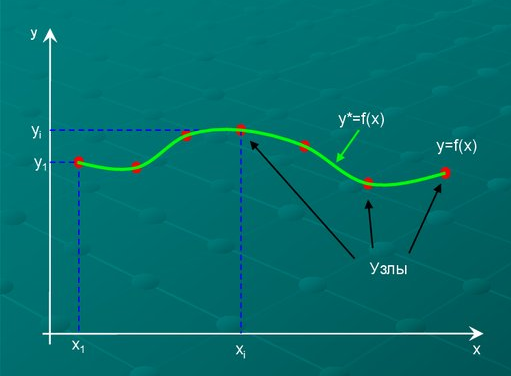
\includegraphics[width=0.65\textwidth]{images/interpolation.png}
					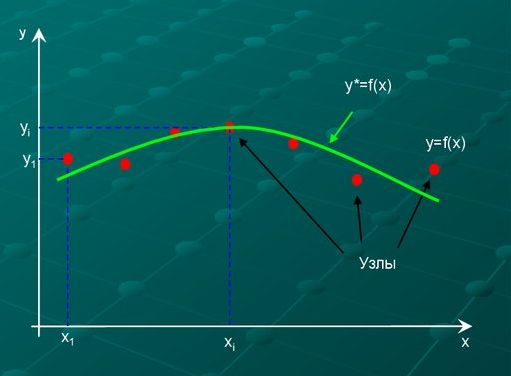
\includegraphics[width=0.65\textwidth]{images/approximation.png}
					\caption {Аппроксимация и интерполяция}
				\end{figure}
			\end{column}
		\end{columns}
			
		\note{

			Основное различие между этими методами заключается в том, где и как они применяются относительно существующего набора данных: 
			\begin{enumerate}
				\item интерполяция работает внутри диапазона, 
				\item аппроксимация стремится к общему соответствию, 
				\item экстраполяция и ретрополяция идут за пределы известного диапазона.
			\end{enumerate}

			% Интерполяция используется для оценки значения функции внутри диапазона наблюдаемых точек данных. Если у нас есть данные о температуре в 10:00 и в 12:00, мы можем использовать интерполяцию, чтобы оценить температуру в 11:00.

			% Аппроксимация – это метод приближения функции, который пытается найти функцию, которая наилучшим образом соответствует всему набору данных, не обязательно точно проходя через каждую точку. Например, метод наименьших квадратов, который пытается минимизировать сумму квадратов отклонений между данными и приближенной функцией.
	
			% Экстраполяция – это процесс оценки значения вне диапазона известных значений. Если у нас есть данные о продажах за последние несколько месяцев, мы можем использовать экстраполяцию, чтобы предсказать продажи в следующем месяце.
	
			% Ретрополяция (менее распространенный термин) аналогична экстраполяции, но оценка производится для точки, которая находится до диапазона имеющихся данных. Например, если у нас есть данные начиная с 2000 года, мы можем использовать ретрополяцию, чтобы оценить какое-то значение в 1995 году.
		}

	\end{frame}



	\section{Сплайн}

	\begin{frame}{Сплайн}
		Слово сплайн (англ. \textquotedbl spline\textquotedbl ) использовалось для обозначения гибких, изогнутых листов дерева или металла, которые могли использоваться в различных инженерных и строительных приложениях.




		
		\note{
			Слово "сплайн" произошло от английского термина "spline". Этот термин, вероятно, образован от слова "сплен" (spline) в шотландском диалекте, которое означает "планка" или "листок дерева". В начале 20 века в англоязычной литературе оно использовалось для обозначения гибких, изогнутых листов дерева или металла, которые могли использоваться в различных инженерных и строительных приложениях.
	
			Слово \textquotedbl сплайн\textquotedbl~было впервые введено в математике и компьютерной графике для обозначения методов интерполяции и аппроксимации кривых, которые используют гладкие сегменты, напоминающие изогнутые листы. Эти методы стали называться \textquotedbl сплайнами\textquotedbl~из-за аналогии с гибкими листами или планками, которые могли быть использованы для создания гладких кривых.

		}

	\end{frame}
	

	\begin{frame}{Общее описание}


		Кусочно-гладкая полиномиальная система --- параметрическая система уравнений.

		Контрольный граф (характеристический многоугольник) --- ломанная линия, соединяющая последовательности точек сплайновой кривой.

		Параметры сплайна
		\begin{itemize}
			\item степень полинома;
			\item положение узловых (или опорных) точек 
		\end{itemize}

		Методы определения сплайна:
		\begin{itemize}
			\item матрица, характеризующая сплайн;
			\item набор базисных функций (стыковочных);
			\item набор граничных условий.
		\end{itemize}

		\note{



		Способы задания и представления

			\begin{columns}
				\begin{column}{0.33\textwidth}
					Явное
					\[
					\begin{cases}
						x = x \\
						y = f(x) \\
						z = g(x) \\
					\end{cases}	
					\]
					Значения новых переменных $y,z$ определяется $x$
				\end{column}
				\begin{column}{0.33\textwidth}
					Неявное
					\[
					\begin{cases}
						f(x,y,z) = 0 \\
						g(x,y,z) = 0 \\
					\end{cases}	
					\]
					Одну из переменных $x,y,z$ не всегда удается выразить.
				\end{column}
				\begin{column}{0.33\textwidth}
					Параметрическое
					\[
					\begin{cases}
						x = x(t) \\
						y = y(t) \\
						z = z(t) \\
					\end{cases}	
					\]
					вводится новая переменная $t$.
				\end{column}
			\end{columns}

		}

	\end{frame}

	\begin{frame}{Матрица, характеризующая сплайн}
		\[
			P(u) = a u^3 + b u^2 + c u + d = U C
		\]
		\[
			\begin{cases}
				P_x(u) = a_x u^3 + b_x u^2 + c_x u + d_x \\
				P_y(u) = a_y u^3 + b_y u^2 + c_y u + d_y \\
				P_z(u) = a_z u^3 + b_z u^2 + c_z u + d_z \\
			\end{cases}
			,
		\]
		где 
		$u \in [0,1]$.
		\note{
			\[
			x(u) = 
			\begin{bmatrix}
				u^3 \\
				u^2 \\
				u \\
				1 \\
			\end{bmatrix}^T
			\begin{bmatrix}
				a_x \\
				b_x \\
				c_x \\
				d_x \\
			\end{bmatrix}
			\qquad
			y(u) = 
			\begin{bmatrix}
				u^3 \\
				u^2 \\
				u \\
				1 \\
			\end{bmatrix}^T
			\begin{bmatrix}
				a_y \\
				b_y \\
				c_y \\
				d_y \\
			\end{bmatrix}
			\qquad
			z(u) = 
				\begin{bmatrix}
					u^3 \\
					u^2 \\
					u \\
					1 \\
				\end{bmatrix}^T
				\begin{bmatrix}
					a_z \\
					b_z \\
					c_z \\
					d_z \\
				\end{bmatrix}
			\]


			\[
				P(u) = U C
			\]
			
			
			% \[
			% 	C = M_s M_g
			% \]
			% где 
			% $M_s$ --- базисная матрица размером $m \times n$, преобразующая граничные условия в коэффициенты;
			% $M_g$ --- матрица столбец, координаты контрольных точек.

		}
	\end{frame}

	\begin{frame}{Граничные условия}

		
		Параметрические условия непрерывности


		\begin{columns}
			\begin{column}{0.6\textwidth}
				\begin{itemize}
					\item 0-го порядка $C^0$ \\
					одинаковые координаты в граничных точках \\
					$P_{j}(1) = P_{j+1}(0)$
					\item 1-го порядка $C^1$ \\
					первые производные пропорциональны в т. пересечения \\
					$P_{j}^{(1)}(1) = P_{j+1}^{(1)}(0)$
					\item 2-го порядка $C^2$ \\
					вторые производные пропорциональны в т. пересечения \\
					$P_{j}^{(2)}(1) = P_{j+1}^{(2)}(0)$
				\end{itemize}
			\end{column}
			\begin{column}{0.4\textwidth}
				\begin{figure} 
					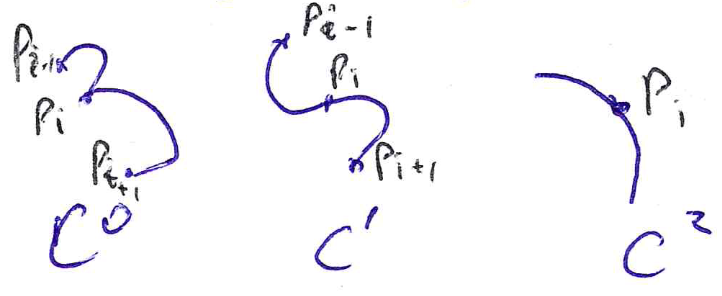
\includegraphics[width=\textwidth]{images/continuity_condition.png}
					\caption {Различие граничных условий}
				\end{figure}
			\end{column}
		\end{columns}

		
		\note{
			Условия геометрической непрерывности
			\begin{itemize}
				\item 0-го порядка $G^0$ \\
				одинаковые координаты в граничных точках \\
				$P_{j}(1) = P_{j+1}(0)$
				\item 1-го порядка $G^1$ \\
				первые производные пропорциональны в т. пересечения \\
				$ \text{sign} \big(P_{j}^{(1)}(1)\big) = \text{sign} \big(P_{j+1}^{(1)}(0)\big)$
				\item 2-го порядка $G^2$ \\
				второе производные пропорциональны в т. пересечения \\
				$ \text{sign} \big(P_{j}^{(2)}(1)\big) = \text{sign} \big(P_{j+1}^{(2)}(0)\big)$
			\end{itemize}

		}

	\end{frame}

	\begin{frame}{Сплайн}{Пространственные кривые}
		Классификация
		\begin{enumerate}
			\item Построение кривых, проходящих через заданные точки
			\begin{enumerate}
				\item Естественный сплайн;
				\item Эрмитов сплайн;
			\end{enumerate}
			\item Построение кривых, заданных направлением изгиба
			\begin{enumerate}
				\item кривая Безье;
				\item B-сплайн.
			\end{enumerate}
		\end{enumerate}

		\note{ 
			Высокая степень полинома приводит к тому, что можно получить сильные колебания ( осцилляции)
		}

	\end{frame}

	\begin{frame}{Естественный сплайн}
		Рассмотрим подробнее, как находить коэффициенты вектора $C_x$.
		\[
			P_x(u) = U C_x
		\]
		\[
			P_x(u) = 
			\begin{bmatrix}
				u^3 \\
				u^2 \\
				u \\
				1 \\
			\end{bmatrix}^T
			\begin{bmatrix}
				a_x \\
				b_x \\
				c_x \\
				d_x \\
			\end{bmatrix}
		\]
		Построим следующую систему уравнений
		\[
			\begin{cases}
				P_{x,i} = P_x(0) = a_x 0^3 + b_x 0^2 + c_x 0 + d_x \\
				P_{x,i+1} = P_x(1/3) = a_x (1/3)^3 + b_x (1/3)^2 + c_x 1/3 + d_x \\
				P_{x,i+2} = P_x(2/3) = a_x (2/3)^3 + b_x (2/3)^2 + c_x 2/3+ d_x \\
				P_{x,i+3} = P_x(1) = a_x 1^3 + b_x 1^2 + c_x 1 + d_x \\
			\end{cases}
		\]

		
		\[
			P_x = A C_x
		\]
		\note{
			\[
				\begin{bmatrix}
					P_{x,i} \\
					P_{x,i+1} \\
					P_{x,i+2} \\
					P_{x,i+3} \\
				\end{bmatrix}
				=
				\begin{bmatrix}
					0 & 0 & 0 & 1 \\
					(1/3)^3 & (1/3)^2 & 1/3 & 1 \\
					(2/3)^3 & (2/3)^2 & 2/3 & 1 \\
					1^3 & 1^2 & 1 & 1 \\
				\end{bmatrix}
				\begin{bmatrix}
					a_x \\
					b_x \\
					c_x \\
					d_x \\
				\end{bmatrix}
			\]
	
			\[
				P_x = A C_x
			\]
			\[
				A^{-1} P_x = A^{-1} A C_x
			\]
			\[
				A^{-1} P_x = E C_x
			\]
			\[
				C_x = A^{-1} P_x
			\]

			\[
				\begin{bmatrix}
					0 & 0 & 0 & 1 \\
					(1/3)^3 & (1/3)^2 & 1/3 & 1 \\
					(2/3)^3 & (2/3)^2 & 2/3 & 1 \\
					1^3 & 1^2 & 1 & 1 \\
				\end{bmatrix}^{-1}
				\begin{bmatrix}
					P_{x,i} \\
					P_{x,i+1} \\
					P_{x,i+2} \\
					P_{x,i+3} \\
				\end{bmatrix}
				=
				\begin{bmatrix}
					a_x \\
					b_x \\
					c_x \\
					d_x \\
				\end{bmatrix}
			\]
		}

	\end{frame}

	\begin{frame}{Эрмитова интерполяция}{Charles Hermite}
		Эрмитов сплайн --- вид кусочно-полиномиальной кривой, которая задается точками данных и значениями производных в этих точках.
		Рассмотрим подробнее, как находить коэффициенты вектора $C_y$.
		\[
			P_y(u) = u^3 a_y + u^2 b_y + u c_y + d_y
		\]

		\[
			(P_y)'_u(u) = P'_y(u) = 3 u^2 a_y + 2 u b_y + c_y + 0
		\]
		
		\[
			\begin{cases}
				P_y(0) = P_{y,k} = 0^3 a_y + 0^2 b_y + 0 c_y + d_y \\
				P_y(1) = P_{y,k+1} = 1^3 a_y + 1^2 b_y + 1 c_y + d_y \\
				P'_y(0) = P'_{y,k} = 3 \cdot 0^2 a_y + 2 \cdot 0 b_y + c_y \\
				P'_y(1) = P'_{y,k+1} = 3 \cdot 1^2 a_y + 2 \cdot 1 b_y + c_y \\
			\end{cases}
		\]



		\note{

		\[
			\begin{bmatrix}
				P_{y,k} \\
				P_{y,k+1} \\
				P'_{y,k} \\
				P'_{y,k+1} \\
			\end{bmatrix}
			=
			\begin{bmatrix}
				0 & 0 & 0 & 1 \\
				1 & 1 & 1 & 1 \\
				0 & 0 & 1 & 0 \\
				3 & 2 & 1 & 0 \\
			\end{bmatrix}
			\begin{bmatrix}
				a_y \\
				b_y \\
				c_y \\
				d_y \\
			\end{bmatrix}
		\]

		\[
			\begin{bmatrix}
				a_y \\
				b_y \\
				c_y \\
				d_y \\
			\end{bmatrix}
			=
			\begin{bmatrix}
				0 & 0 & 0 & 1 \\
				1 & 1 & 1 & 1 \\
				0 & 0 & 1 & 0 \\
				3 & 2 & 1 & 0 \\
			\end{bmatrix}^{-1}
			\begin{bmatrix}
				P_{y,k} \\
				P_{y,k+1} \\
				P'_{y,k} \\
				P'_{y,k+1} \\
			\end{bmatrix}
		\]

		\[
			\begin{bmatrix}
				a_y \\
				b_y \\
				c_y \\
				d_y \\
			\end{bmatrix}
			=
			\begin{bmatrix}
				2 & -2 & 1 & 1 \\
				-3 & 3 & -2 & -1 \\
				0 & 0 & 1 & 0 \\
				1 & 0 & 0 & 0 \\
			\end{bmatrix}
			\begin{bmatrix}
				P_{y,k} \\
				P_{y,k+1} \\
				P'_{y,k} \\
				P'_{y,k+1} \\
			\end{bmatrix}
		\]
		}

	\end{frame}

	\begin{frame}{Сплайновые кривые Безье}{Pierre Bezier}

		Кривая Безье --- это математическое представление кривой, определенной с использованием параметрических уравнений.

		\[
			P_n(u) = \sum_{k = 0}^{n}	P_k B_k(u)
			,
		\]
		где 
		
		$B_k (u)$ --- глобальный базис;

		$P_k$ --- узловые точки;

		
		$n$ --- степень полинома;

		$u \in [0,1]$.

		\[
			B_k (u) = C_n^k u^k (1 - u)^{n-k}	
		\]
		Примечание. \\ Формула основана на биноме Ньютона

		\note{
			\begin{figure} 
				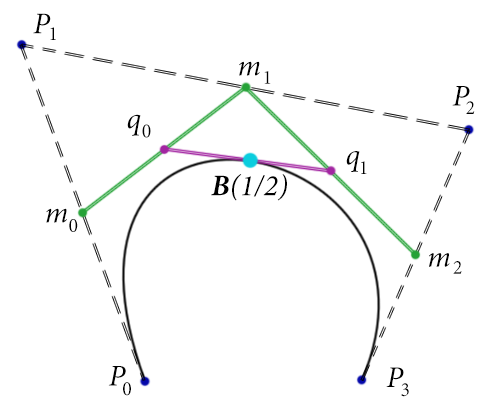
\includegraphics[width=0.6\textwidth]{images/Bezier_spline.png}
			\caption{Схема построения кривой Безье}
		\end{figure}
		}

	\end{frame}

	\begin{frame}{Сплайновые кривые Безье}{Пример}


		\[
			n = 1	
		\]
		\[
			P(u) = P_0 C_1^0 u^0 (1-u)^1 + P_1 C_1^1 u^1 (1-u)^0 
		\]
		\[
			P(u) = P_0 (1-u) + P_1  u = P_0 + (P_1 - P_0) u
		\]

		\[
			n = 2
		\]
		\[
			P(u) = P_0 C_2^0 u^0 (1-u)^2 + P_1 C_2^1 u^1 (1-u)^1 + P_2 C_2^2 u^2 (1-u)^0 
		\]
		\[
			P(u) = P_0 (1-u)^2 + 2 P_1 u (1-u) + P_2  u^2
		\]

		\[
			n = 3
		\]
		\[
			P(u) = P_0 (1-u)^3 + P_1 3 u (1-u)^2 + P_2 3 u^2 (1-u) + P_3 u^3
		\]
		\[
			P(u) = P_0 (1-u)^3 + P_1 3 u (1-u)^2 + P_2 3 u^2 (1-u) + P_3 u^3 
		\]
		

		\note{
			{ \footnotesize
			Свойства
			\begin{itemize}
				\item Локальный контроль: Изменения в контрольных точках кривой Безье оказывают влияние только на ограниченный сегмент кривой, что делает её легко управляемой.

				\item Степень кривой: Степень кривой Безье определяется числом контрольных точек минус один. Таким образом, для $n+1$ точек степень кривой будет $n$.
		
				\item Инвариантность относительно линейных преобразований: Кривые Безье сохраняют свою форму при линейных преобразованиях, таких как сжатие, вращение и перенос.
		
				\item Выпуклость: Кривые Безье всегда остаются в пределах выпуклой оболочки своих контрольных точек (глобальный базис).
		
				\item  Касательные в начальной и конечной точках: Касательные к кривой в начальной и конечной точках совпадают с линиями, соединяющими соответствующие контрольные точки.
			\end{itemize}
			}
		}

	\end{frame}

	\begin{frame}{B-сплайн}{B-spline}
		B-сплайн  --- кусочно-полиномиальная кривая, определенная с использованием базисных функций.

		\[
			P_k(u) = \sum_{i=0}^{n} P_i N_{i, k} (t)
			,	
		\]
		где 
		$N_{i,k}(t)$ --- локальный базис;
		$P_i$ --- узловые точки;
		\\ $k$ --- степень полинома;
		$t \in  [t_{min}; t_{max})$.

		

		Рекуррентные формулы Кокса-де Бура %(Гордона-Ризенфельда)
		\[
		N_{i,0} (t) =
		\begin{cases}
			1, & \text{если~} t \in  [t_{i}; t_{i+1}) \\
			0, & \text{иначе} \\
		\end{cases}	
		\]

		\[
			N_{i,k} (t) =
			N_{i,k-1} (t)
			\frac{t - t_i}{t_{i+k} - t_i} 
			+
			N_{i+1,k-1} (t)
			\frac{t_{i+1+k} - t}{t_{i+1+k} - t_{i+1}} 
		\]

		\note{

		\begin{figure} 
			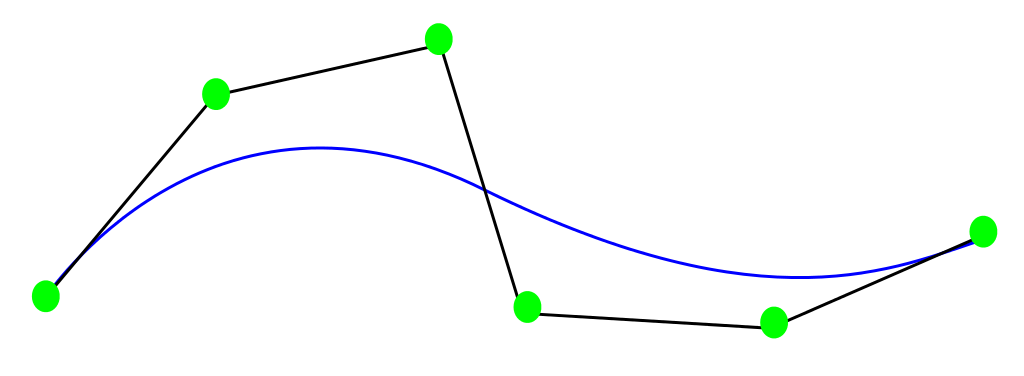
\includegraphics[width=\textwidth]{images/B-spline.png}
		\caption{B-spline}
	\end{figure}
		}

\end{frame}

	\begin{frame}{B-сплайн}{Пример}

		Пусть даны три точки $P_0$,$P_1$,$P_2$ и вектор $T = [t_0, t_1, \dots, t_i, \dots,t_5]$, где $t_i\leqslant t_{i+1}$.

			\begin{table}
				% \caption{\label{tab:fractal} Название}
				\begin{center}
					\begin{tabular}{|c|c|c|c|c|}
						\hline
						$x$ & $l$ & $2$ & $4$ \\
						\hline
						$y$ & $l$ & $3$ & $3$ \\
						\hline
					\end{tabular}
				\end{center}
			\end{table}

			\[
				T=[0,0,1,2,3,3]	
			\]

			
			Тогда
			
			$ n + 1 = 3$ --- число узловых точек;

			$m +1 = 6$ --- число  элементов вектора T;

			$m - (n+1) = 2$ --- степень полинома.

			Схема
			\[
				\begin{array}{l l c}
				\text{константы}	& N_{i,0} & N_{0,0} \quad N_{1,0} \quad N_{2,0} \quad N_{3,0} \quad N_{4,0} \\
				\text{полином 1-й степени}  &	N_{i,1} & N_{0,1} \quad N_{1,1} \quad N_{2,1} \quad N_{3,1} \\
				\text{полином 2-й степени} &	N_{i,2} & N_{0,2} \quad N_{1,2} \quad N_{2,2} \\
				\end{array}
			\]

			\note{
		\[
			N_{0,0} = 0 
			\]
			\[
				N_{1,0} = 1, t \in [0,1)
			\]
			\[
				N_{2,0} = 1, t \in [1,2) 
			\]
		\[
			N_{3,0} = 1, t \in [2,3) 
			\]
			\[
				N_{4,0} = 0
			\]

		\[
			N_{0,1} (t) 
			= 
			N_{0,0}(t) 
			\frac{t - t_0}{t_1 - t_0} 
			+ 
			N_{1,0}(t) 
			\frac{t_2 - t}{t_2 - t_1} 
			=
		\] 
		\[
			=
			\begin{cases}
				0
				\cdot 
				\frac{t}{0} 
				, & t \in [0,0) \\
				1
				\cdot 
				\frac{1 - t}{1} 
				, & t \in [0,1) \\	
			\end{cases}
			= 
			\begin{cases}
			0, & t \in [0,0) \\
			1-t, & t \in [0,1) \\	
			\end{cases}
		\]
		\[\cdots\]

			}
		

	\end{frame}

	\begin{frame}{B-сплайн}{Пример}
		\[
			P(t) = P_0 N_{0,2}(t) + P_1 N_{1,2}(t) + P_2 N_{2,2}(t) 
		\]

		% \[
		% 	P(t) = (1 - t) P_1 + t P_2 
		% \]

		% \[
		% 	P(t) = (1 - t) P_1 + t P_2 
		% \]


		\note{
			Свойства:
			{ \scriptsize
			\begin{itemize}
				\item 
				Сумма $\sum_{n}^{i=0} N_{i,k} (t) \equiv 1$;
				$N_{i,k} (t) \geqslant 0$ при $\forall t \in [t_{min}, t_{max}]$;
				\item 
				Перемещение: чтобы применить к кривой любое аффинное преобразование необходимо применить его к вершинном определяющая многоугольника;
				\item
				Кусочная гладкость: обеспечивают гладкость на границах сегментов и обеспечивают непрерывность определенного порядка на всей кривой.
				\item
				Локальная модификация: Изменения в контрольных точках B-сплайна оказывают влияние только на ограниченный сегмент кривой, что делает их удобными для локальных модификаций.
				\item
				Вариативность степени и узлов: могут иметь разные степени и распределение узлов, что позволяет легко адаптировать их к различным требованиям.
				\item
				Контроль над кривой: Контроль над формой кривой обеспечивается не только контрольными точками, но и базисными функциями, что делает их более гибкими.
				% \item
				% Интерполяция и аппроксимация: могут использоваться для интерполяции или аппроксимации с использованием контрольных точек и базисных функций.
			\end{itemize}
		}
		}
	\end{frame}

	\end{document}

	\[
		\begin{bmatrix}
			1 & 0 & 0 & 0 \\
			0 & 1 & 0 & 0 \\
			0 & 0 & 1 & 0 \\
			-\frac{left + right}{2} & -\frac{bottom + top}{2} & 0 & 1 \\
		\end{bmatrix}	
	\]
	
	% https://learnwebgl.brown37.net/08_projections/projections_ortho.html
	% https://www.songho.ca/opengl/gl_projectionmatrix.html
	% https://www.scratchapixel.com/lessons/3d-basic-rendering/perspective-and-orthographic-projection-matrix/opengl-perspective-projection-matrix.html
	% https://en.wikipedia.org/wiki/Viewing_frustum
	% https://www.reddit.com/r/opengl/comments/2hs6cf/questionglmfrustum_or_glmperspective/
	% https://startandroid.ru/ru/uroki/vse-uroki-spiskom/401-urok-172-perspective-frustum-ortho.html
	% http://doc.51windows.net/Directx9_SDK/graphics/programmingguide/fixedfunction/viewportsclipping/viewingfrustum.htm
	% https://www.google.com/search?q=camera+transformation+FOV&tbm=isch&ved=2ahUKEwjh6-yX7_CBAxXwBxAIHS7gDtwQ2-cCegQIABAA&oq=camera+transformation+FOV&gs_lcp=CgNpbWcQAzoHCAAQigUQQzoFCAAQgAQ6BggAEAgQHjoHCAAQGBCABDoECAAQHlDSAlizDWDWDmgBcAB4AIABUYgBwwKSAQE2mAEAoAEBqgELZ3dzLXdpei1pbWfAAQE&sclient=img&ei=mxYoZaGyMvCPwPAPrsC74A0&bih=921&biw=1920#imgrc=1JjqcwhhFgAhiM



	\begin{figure} 
		\href{https://www.researchgate.net/figure/Outline-of-the-graphics-pipeline_fig1_281810652}{
			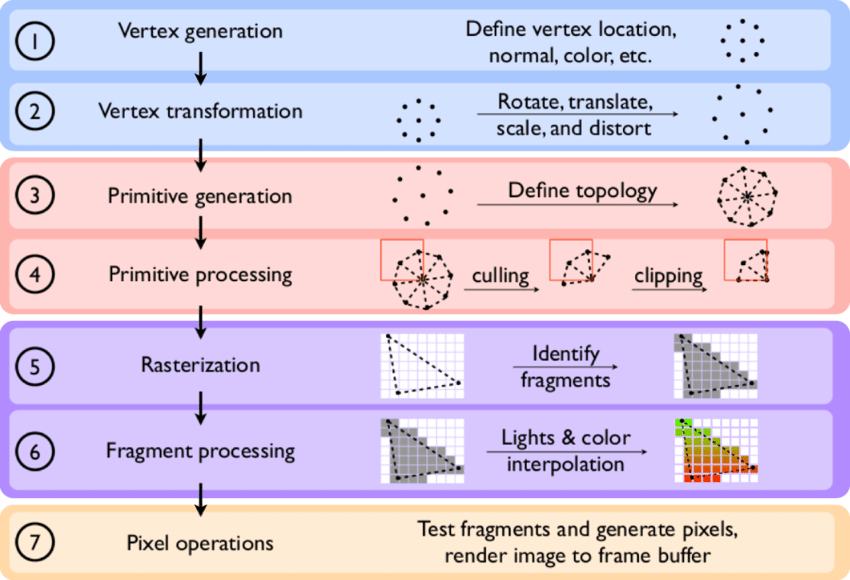
\includegraphics[width=0.75\textwidth]{images/Outline-of-the-graphics-pipeline.png}}
		\caption{Схема графического конвейера}
	\end{figure}

	\begin{figure} 
			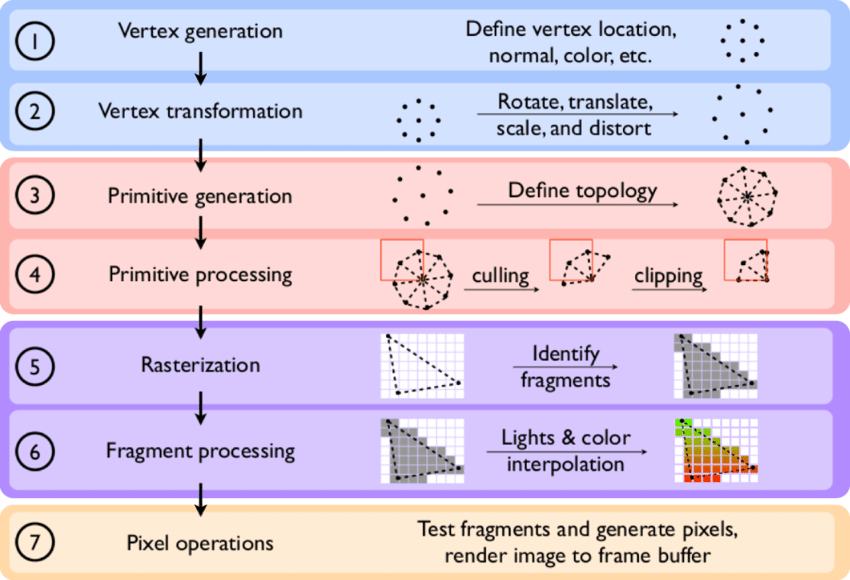
\includegraphics[width=0.75\textwidth]{images/Outline-of-the-graphics-pipeline.png}
		\caption{Схема графического конвейера}
	\end{figure}

	\begin{columns}
		\begin{column}{0.5\textwidth}
			\begin{figure} 
				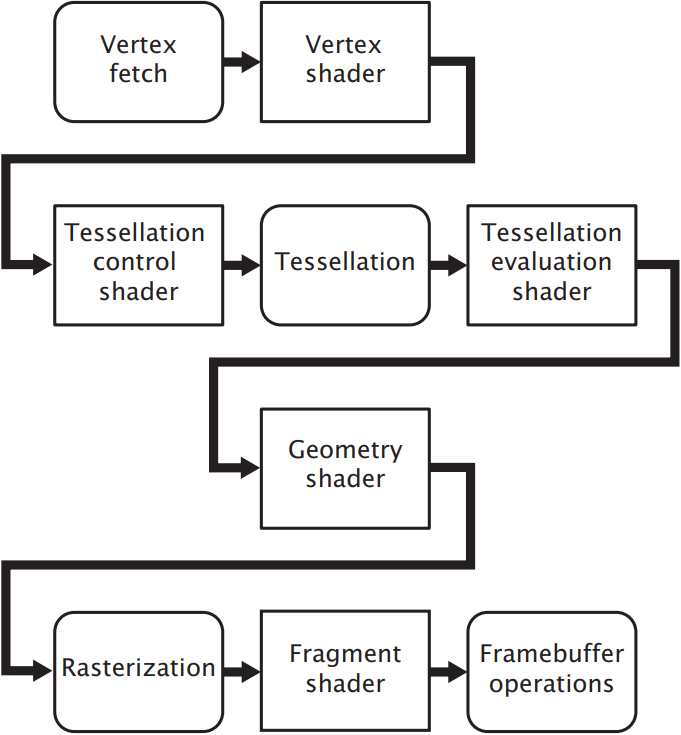
\includegraphics[width=0.9\textwidth]{images/Simplified_model_of_the_graphics_pipeline.png}
				\caption {Порядок вычисления шейдеров}
			\end{figure}
		\end{column}
		\begin{column}{0.5\textwidth}
		\end{column}
	\end{columns}
			

			\footnotesize

			\begin{table}
				% \caption{\label{tab:fractal} Название}
				\begin{center}
					\begin{tabular}{|c|c|c|}
						\hline
						$k$ & $l$ & $N(l)$ \\
						\hline
						0 & $1$ & $1$ \\
						\hline
						1 & $1/2$ & $3$ \\
						\hline
						2 & $1/4$ & $9$ \\
						\hline
						\multicolumn{3}{|c|} {\dots} \\
						\hline
						n & $2^{-n}$ & $3^{n}$ \\
						\hline
					\end{tabular}
				\end{center}
			\end{table}